\documentclass[paper=a4, fontsize=11pt]{scrartcl}

%\usepackage[T1]{fontenc} 
\usepackage[english]{babel} 
\usepackage{amsmath}
\usepackage{amsfonts}
\usepackage{amsthm}
\usepackage{amssymb}
\usepackage{changepage}
\usepackage{titlesec}
\usepackage{subcaption}
\usepackage{xspace}
\newcommand{\MATLAB}{\textsc{Matlab}\xspace}
\usepackage{sectsty} 
\usepackage{graphicx} 

\sectionfont{\centering \normalfont \scshape}
\subsectionfont{\normalfont}
\subsubsectionfont{\normalfont}

\usepackage{fancyhdr} 
\pagestyle{fancyplain} 
\fancyhead{} 
\fancyfoot[L]{} 
\fancyfoot[R]{} 
\fancyfoot[C]{\thepage} 
\renewcommand{\headrulewidth}{0pt} 
\renewcommand{\footrulewidth}{0pt} 
\setlength{\headheight}{13.6pt} 

\usepackage{enumitem}
\newcommand{\subscript}[2]{$#1 _ #2$}
\newcommand*\dif{\mathop{}\!\mathrm{d}}
\newcommand{\pder}[2]{\frac{\partial #1}{\partial #2}}   
\newcommand{\nextline}{$ $ \newline \vspace{-0.15in}}
\newcommand{\horrule}[1]{\rule{\linewidth}{#1}} 

\newcommand{\overbar}[1]{
	\mkern 1.5mu \overline{\mkern-1.5mu\raisebox{0pt}[\dimexpr\height+0.5mm\relax]{$#1$}\mkern-1.5mu}\mkern 1.5mu
}

%------------------------------
\title{	
	\normalfont \normalsize 
	\textsc{Konkuk University Dept. of Physics} \\ [25pt] %Konkuk University Dept. of Physics
	\horrule{1pt} \\[0.4cm] 
	\huge Numerical Analysis Assignment \\
	\vspace{0.1in}
	\Large 2019 Spring Semester
	\horrule{1pt} \\[0.4cm] 
}
\author{Youngwan Kim} 
\date{\normalsize\today} 
%------------------------------
\newtheorem*{ass}{Assignment}

\DeclareCaptionFont{white}{\color{white}}
\DeclareCaptionFormat{listing}{\colorbox{gray}{\parbox{\textwidth}{#1#2#3}}}
\captionsetup[lstlisting]{format=listing,labelfont=white,textfont=white}

%---------------------------------
\usepackage{listings}
\usepackage{inconsolata}
\usepackage{xcolor}
%\usepackage{courier}
\usepackage{color} %red, green, blue, yellow, cyan, magenta, black, white
\definecolor{mygreen}{RGB}{28,172,0} % color values Red, Green, Blue
\definecolor{mylilas}{RGB}{170,55,241}

\lstset{
	basicstyle=\ttfamily,
	language=Matlab,%
	%basicstyle=\color{red},
	breaklines=true,%
	morekeywords={matlab2tikz},
	keywordstyle=\color{blue},%
%	morekeywords=[2]{1}, keywordstyle=[2]{\color{black}},
%	identifierstyle=\color{black},%
	stringstyle=\color{mylilas},
	commentstyle=\color{mygreen},%
%	showstringspaces=false,%without this there will be a symbol in the places where there is a space
	numbers=left,%
	numberstyle={\tiny \color{black}},% size of the numbers
%	numbersep=5pt, % this defines how far the numbers are from the text
	emph=[1]{for,end,break},emphstyle=[1]\color{red}, %some words to emphasise
%	%emph=[2]{word1,word2}, emphstyle=[2]{style},   
}

%---------------------------------
\begin{document}
	
\maketitle	


\begin{ass}
	Implement a \MATLAB code in order to plot a Bezier curve using the second method introduced during the class.
\end{ass}

\vspace{0.15in}

 In total there are 3 \MATLAB script files. The main routine for the code is implemented in \texttt{bezier\_hw.m}, and the other \MATLAB scripts are implementations of functions including \texttt{Mid(P,n)} and \texttt{Bzrt(n)}. Before introducing the main routine, let us go through the functions first.  \\

\begin{lstlisting}[caption='Mid.m']
function Mid=Mid(P)

Mid = [  P(1,:); 
	(P(1,:)+P(2,:))/2 ; 
 	(P(1,:)+2*P(2,:)+P(3,:))/4 ; 
 	(P(1,:)+3*P(2,:)+3*P(3,:)+P(4,:))/8 ;
 	(P(1,:)+3*P(2,:)+3*P(3,:)+P(4,:))/8 ;
 	(P(2,:)+2*P(3,:)+P(4,:))/4 ; 
 	(P(3,:)+P(4,:))/2 ;
 	 P(4,:) ];
\end{lstlisting}
\vspace{0.15in}

The above \texttt{Mid(P)} function gets a \texttt{4$\times$2} matrix as an input, where each of the \texttt{P(i,:)} of \texttt{P} are a single control point. Thus \texttt{Mid(P)} gets 4 control points of a Bezier curve as an input, and it gives us an output of a \texttt{8$\times$2} matrix, or 8 points. These 8 points will act as new control points for the half-segments of the initial Bezier curve given. To elaborate, \texttt{Mid(P)(1:4,1:2)} will be the control points for $B(\frac{t}{2})$ and \texttt{Mid(P)(5:8,1:2)} for $B(\frac{1+t}{2})$ where $B(t)$ is the Bezier curve defined by \texttt{P} and for $t \in [0,1]$.\\

Here I deliberately duplicated the midpoint in order to ease indexing problems later. (This might have caused some unnecessary computations)\\

\begin{lstlisting}[caption='Bzrt.m']
function Bzrt(P,n)

for i=1:n
 for j=1:2^(i-1)
  Q(8*j-7:8*j,1:2) = Mid(P(4*j-3:4*j,1:2));
 end
P=Q;
end

plot(P(:,1),P(:,2),'o-')
\end{lstlisting}
\vspace{0.15in}

The above function \texttt{Bzrt(P,n)} has 2 inputs, where \texttt{P} again is the control points of the Bezier curve. Also \texttt{n} is an input parameter which will act as the desired accuracy for approximation, or the desired number of iterations. The relation used in the code is a generalization of a recursion I discovered while writing this code : \\

\begin{verbatim}
i=1 1
P(1:8,1:2)=Mid(P(1:4,1:2))

i=2 2 2^1
P(1:8,1:2)=Mid(P(1:4,1:2))
P(9:16,1:2)=Mid(P(5:8,1:2))

i=3 4 2^2
P(1:8,1:2)=Mid(P(1:4,1:2))
P(9:16,1:2)=Mid(P(5:8,1:2))
P(17:24,1:2)=Mid(P(9:12,1:2))
P(25:32,1:2)=Mid(P(13:16,1:2))
\end{verbatim}

and so on. After getting the points the code plots the final points. The code itself requires a double for loop in order to obtain $2^{(n+2)}$ points to approximate the Bezier curve. The following is a result of a test script to see if the code above works well : \\

\begin{figure}[htb]
\centering
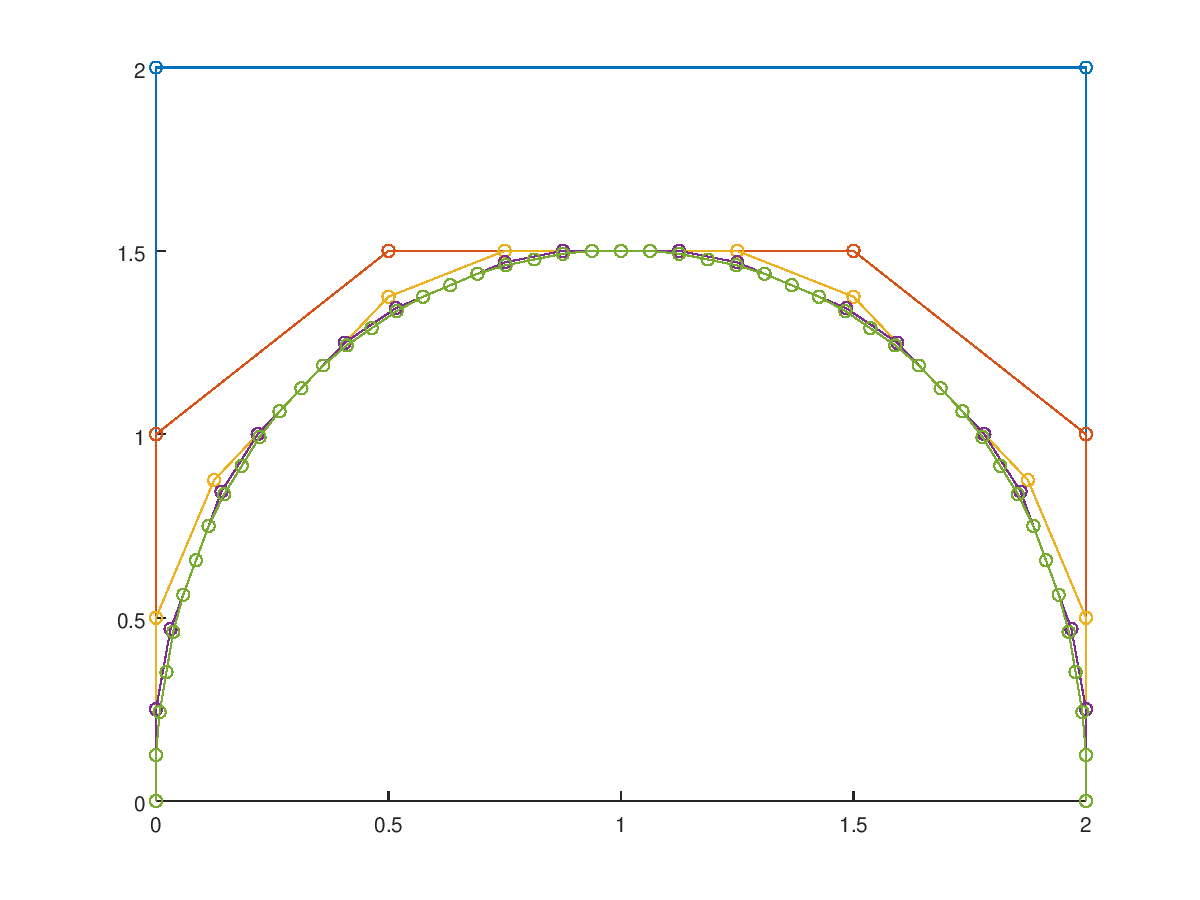
\includegraphics[width=250px]{./img/test4.png}
\end{figure}

The control points used here for testing the code was $(0,0)$, $(0,2)$, $(2,2)$ and $(2,0)$. Also starting from the outside the control parameter was set as $n=0$ to $n=4$. We can obviously see that as $n$ gets bigger the more closer it gets to the desired Bezier curve.\\

\begin{lstlisting}[caption='bezier\_hw.m']
function bezier_hw(n)
figure; hold on
axis([1 700 0 700])
load T.txt

for i=1:size(T,1)
 for j=1:4
  P(j,:)=T(i,:)(2*j-1:2*j);
 end
Bzrt(P,n);
end
\end{lstlisting}
\vspace{0.15in}

Now we take a look at the main routine code \texttt{bezier\_hw.m}, which is also a function as it gets an input \texttt{n}, which is a parameter for approximation accuracy. This code loads a \texttt{16$\times$8} matrix by loading \texttt{T.txt}. Each \texttt{T(i,:)} has 8 coordinate information of the 4 control points for a single Bezier curve, in total having 16 Bezier curves to express T. The first routine goes through these 16 Bezier curves. The inner routine (lines 7 to 9) is a simple code converting a \texttt{1$\times$8} matrix into a \texttt{4$\times$2} matrix in order to fit it into \texttt{Mid(P)} and \texttt{Bzrt(P,n)}. After reshaping \texttt{T(i,:)} into \texttt{P}, for each \texttt{T(i,:)} it evaluates and plots the $2^{(n+2)}$ points of approximation using the \texttt{Bzrt(P,n)} function. The \texttt{figure; hold on} code lets the 16 set of line segments plotted in a single figure. \\


Here is the final result of approximating the Bezier curve data of \texttt{T.txt} into line segments : \\

\begin{figure}[htb]
	\centering
	\begin{subfigure}{0.3\textwidth}
		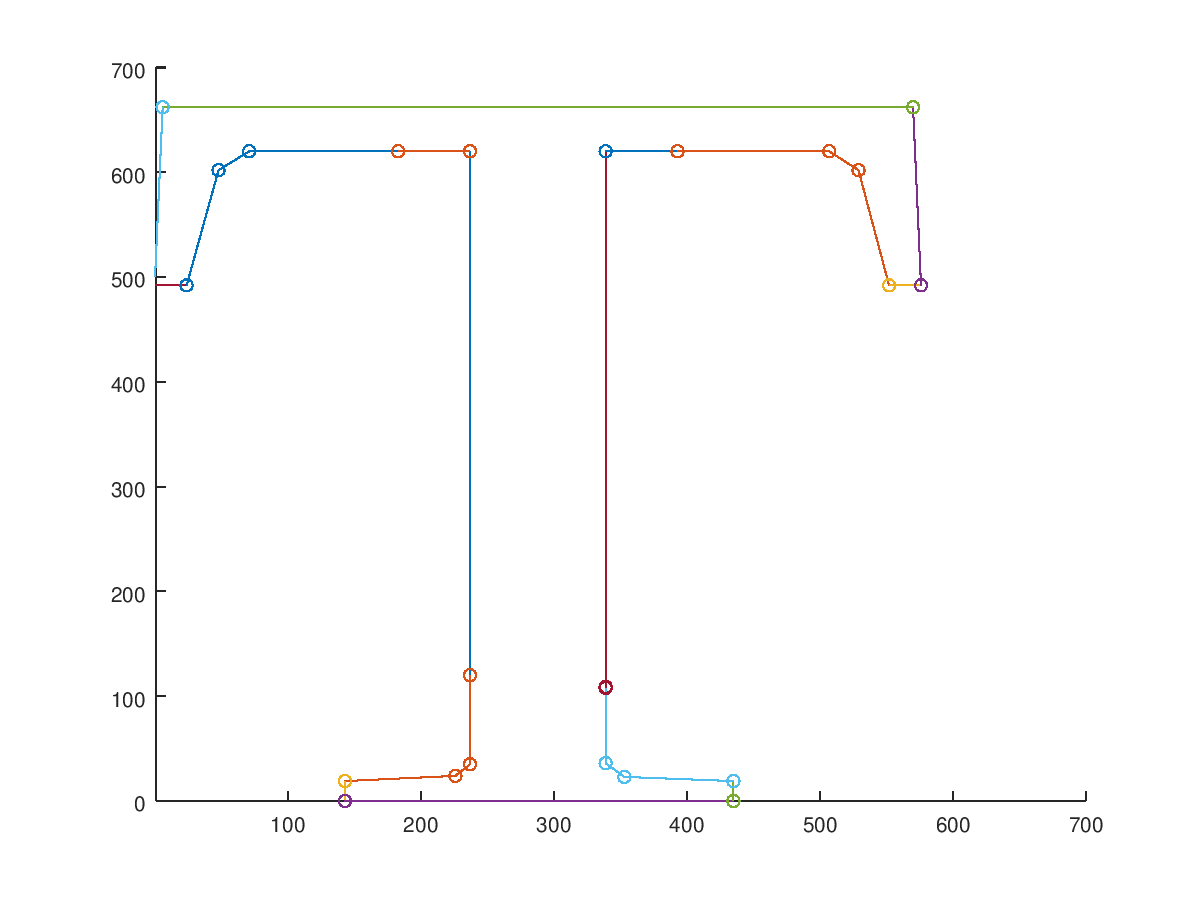
\includegraphics[width=125px]{./img/hw0.png}
		\caption{$n=0$}
	\end{subfigure}\hfil % <-- added
	\begin{subfigure}{0.3\textwidth}
		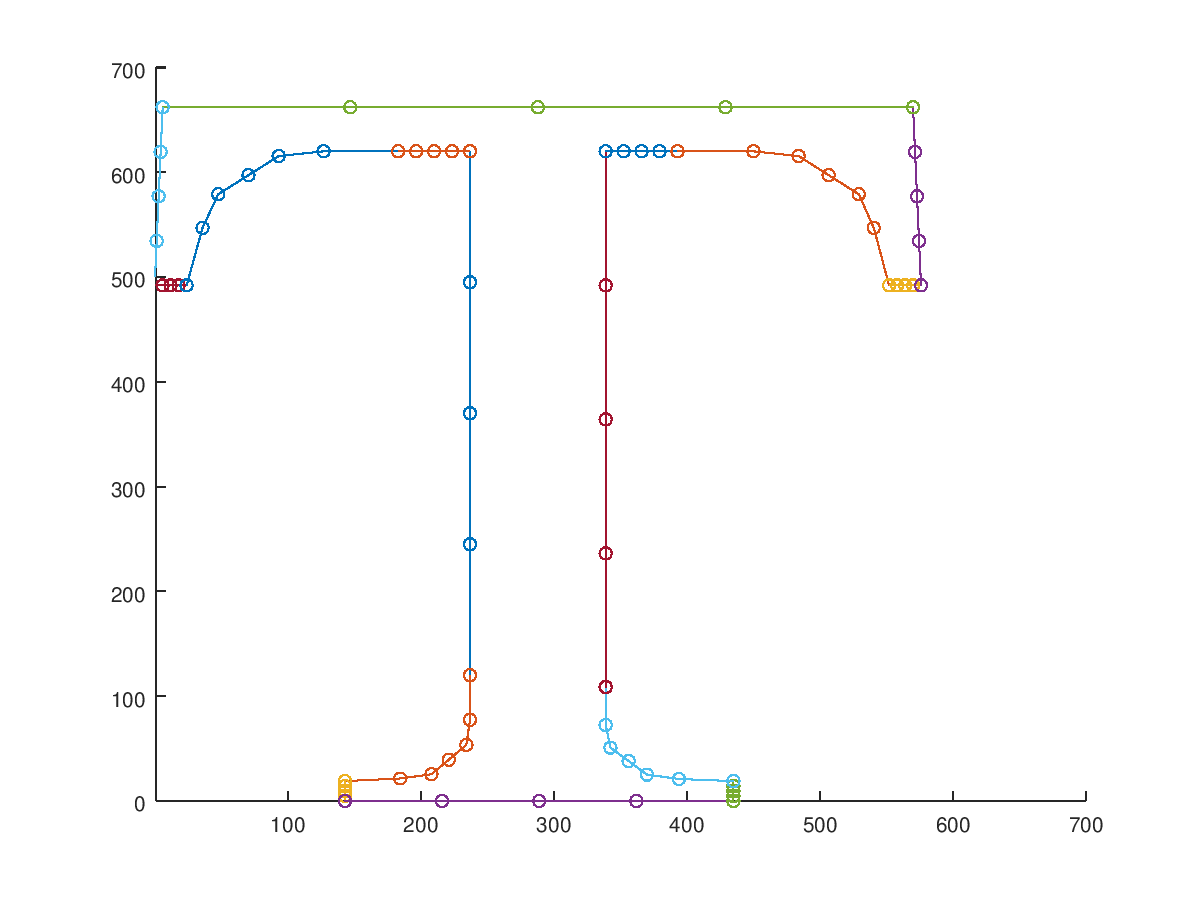
\includegraphics[width=125px]{./img/hw1.png}
		\caption{$n=1$}
	\end{subfigure}\hfil % <-- added
	\begin{subfigure}{0.3\textwidth}
		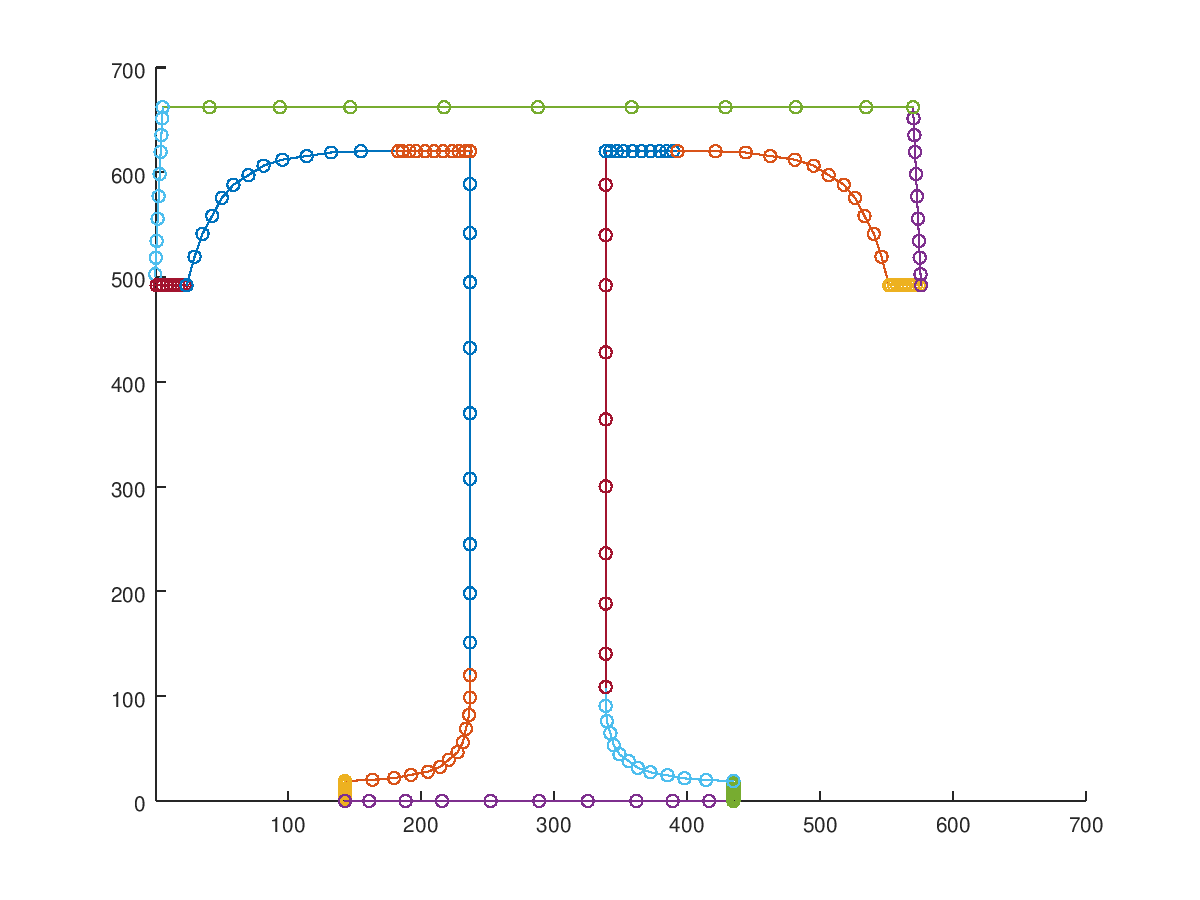
\includegraphics[width=125px]{./img/hw2.png}
		\caption{$n=2$}
	\end{subfigure}\hfil
	\begin{subfigure}{0.3\textwidth}
	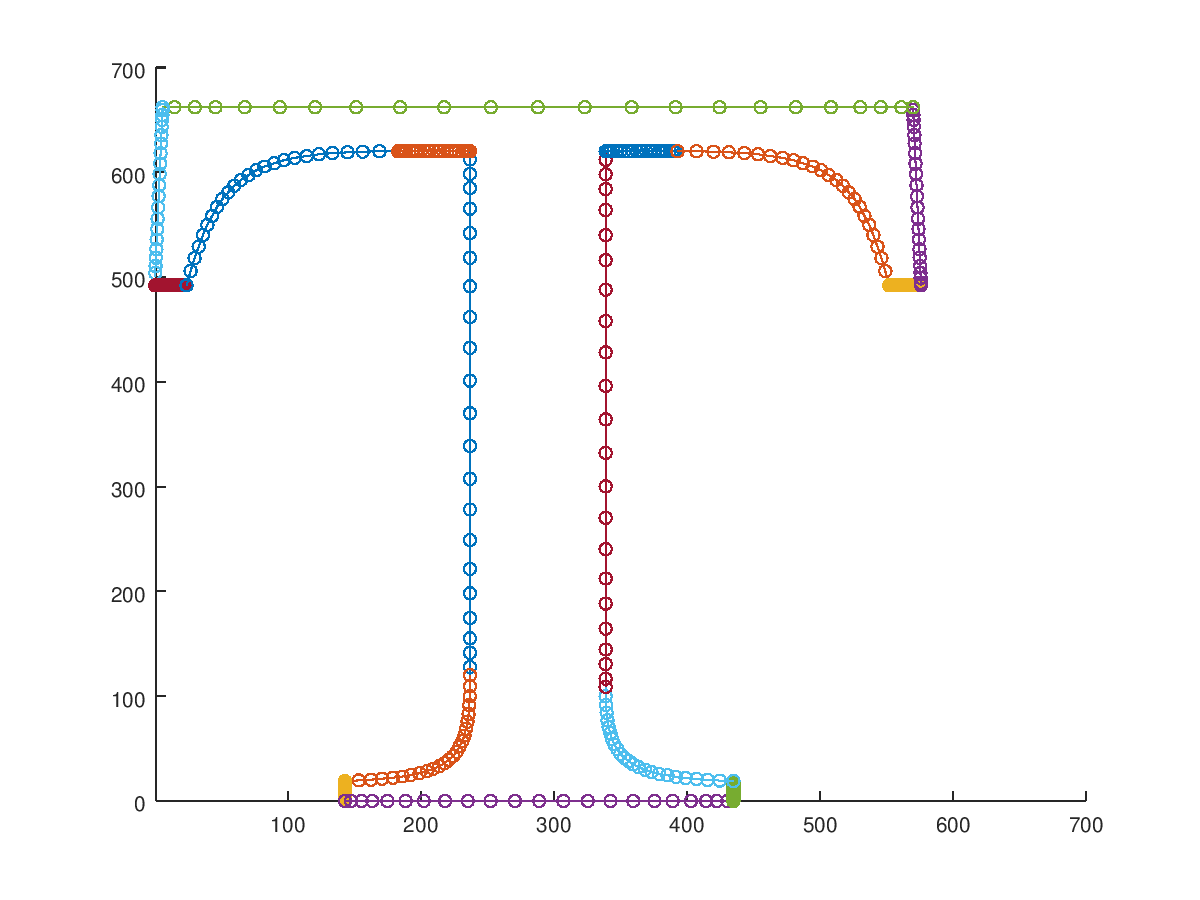
\includegraphics[width=125px]{./img/hw3.png}
	\caption{$n=3$}
	\end{subfigure}\hfil
	\begin{subfigure}{0.3\textwidth}
	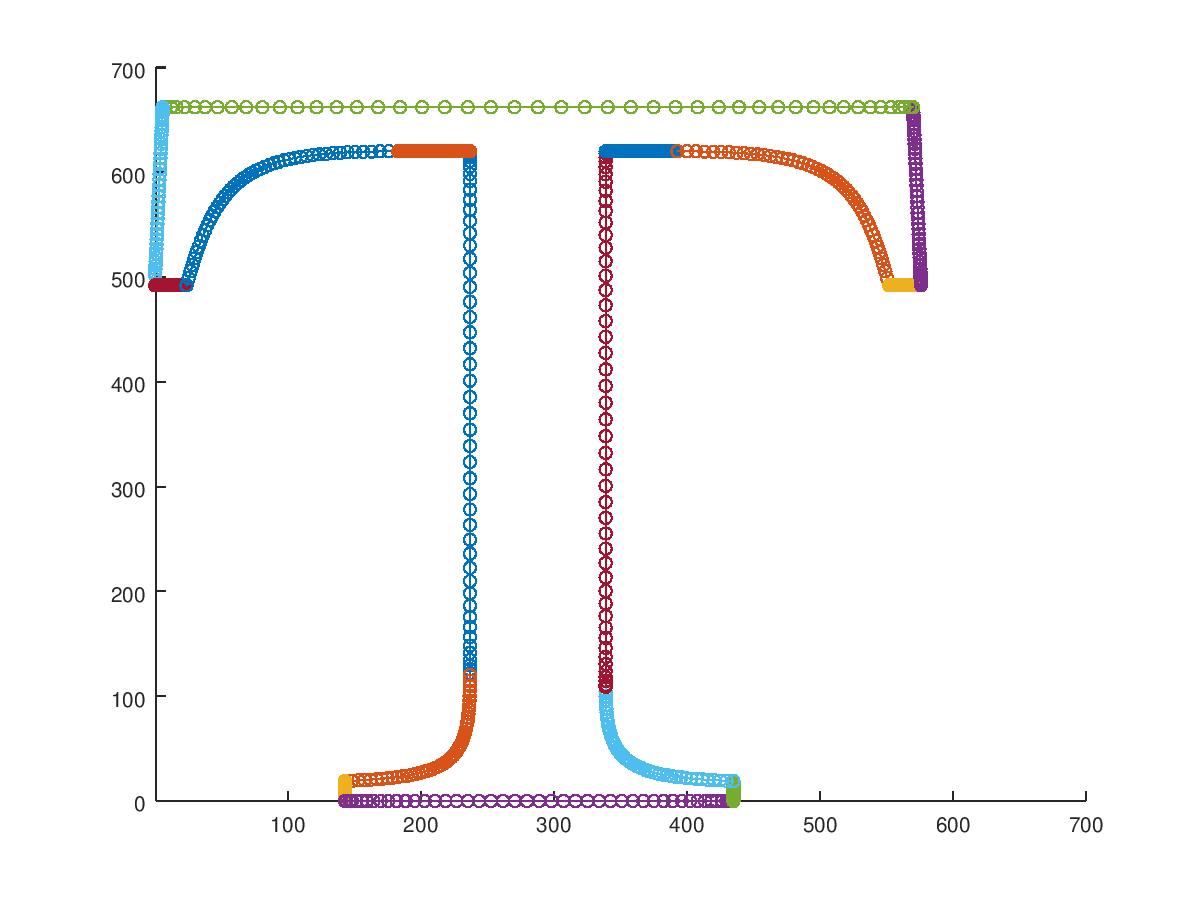
\includegraphics[width=125px]{./img/hw4.png}
	\caption{$n=4$}
	\end{subfigure}\hfil
	\begin{subfigure}{0.3\textwidth}
	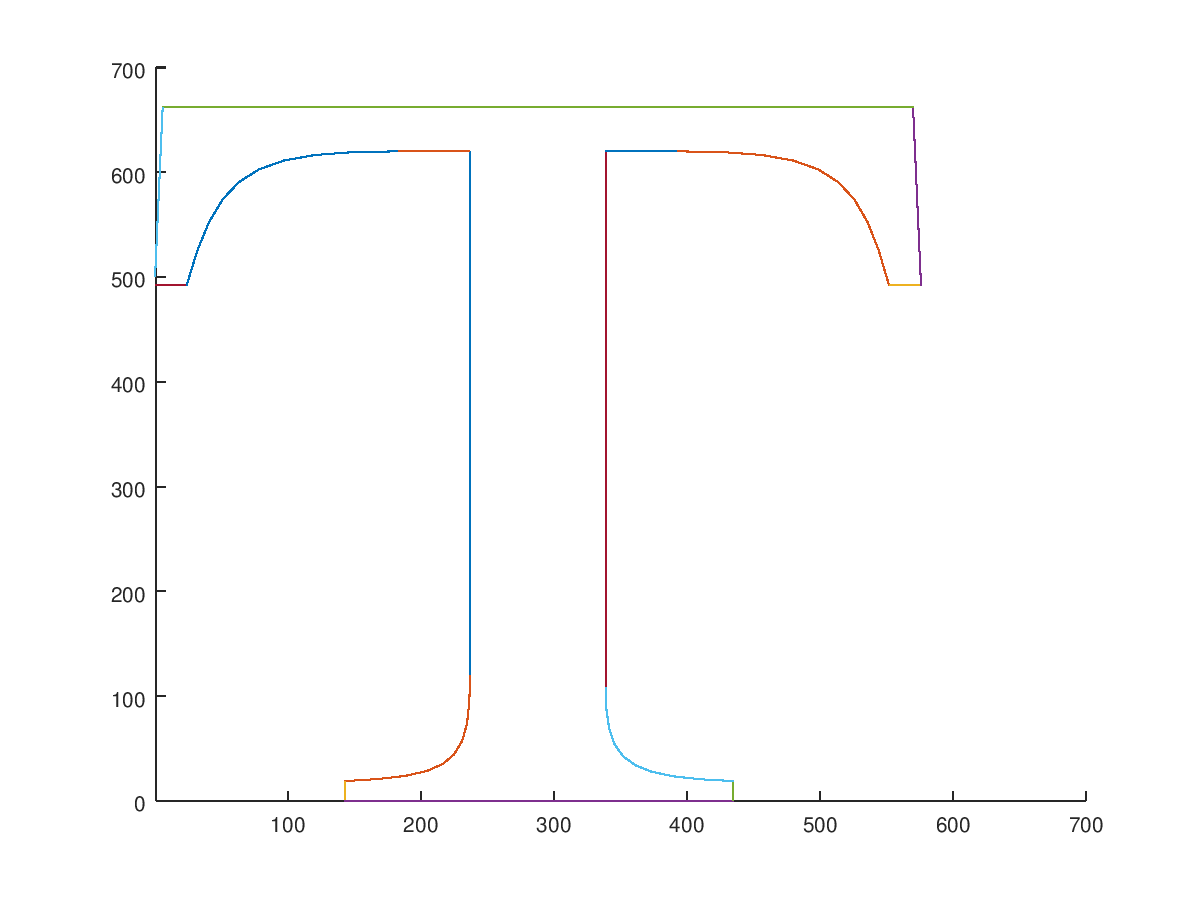
\includegraphics[width=125px]{./img/real.png}
	\caption{real Bezier curve}
	\end{subfigure}\hfil
\end{figure}
\end{document}